\documentclass[9pt, oneside]{extarticle}   	% use "amsart" instead of "article" for AMSLaTeX format
%\usepackage{geometry}                		% See geometry.pdf to learn the layout options. There are lots.
%\geometry{letterpaper}                   		% ... or a4paper or a5paper or ... 
\usepackage[pass,letterpaper]{geometry}
%\geometry{landscape}                		% Activate for for rotated page geometry
\usepackage{graphicx}				% Use pdf, png, jpg, or eps� with pdflatex; use eps in DVI mode
								% TeX will automatically convert eps --> pdf in pdflatex								
\usepackage{amssymb}
\usepackage{tikz,adjust box}			%adjustbox is for figures that span 2 columns
\usepackage{dashrule}				%used to make dashed line in text
\usepackage{amsmath}
\DeclareMathOperator{\arcsec}{arcsec}	%arcsec, arccsc... not defined inamsmath
\usepackage{exsheets}				%Formats questions and solutions
\usepackage{title sec}				%Format section titles to include horizontal line
\titleformat{\section}
  {\normalfont\Large\bfseries}{\thesection}{1em}{}[{\titlerule[0.8pt]}]
\newcommand{\calc}{\protect\includegraphics[height = 2.5ex]{images/calc.png}}  

\title{Problem Solving}
\author{PHS}
%\date{}							% Activate to display a given date or no date
\begin{document}
%\maketitle

\begin{verbatim}
%%%%%%%%ExportDiagram%%%%%%%%%%
\documentclass{standalone}
\usepackage{tikz}

\begin{document}

\begin{tikzpicture}
	\draw [step=0.5] (-1.4,-1.4) grid (1.4,1.4);
\end{tikzpicture}
\end{document}
The new version 1.0 standalone now has the ability to call the above command line (and others) automatically, e.g.:
\documentclass[convert={density=300,size=1080x800,outext=.png}]{standalone}
or simply (using default setting 300dpi, no resizing, PNG):
\documentclass[convert]{standalone}
This needs the -shell-escape compiler option to allow the execution of the conversion program from within the LaTeX document.
%%%%%%%%%%%%%%%%%%%%%%%%%
\end{verbatim}
\hrule

\begin{verbatim}
%%%%%%%%reference a question%%%%%%%%%
\begin{question}[class=medium]\label{cont}
\ref{cont}
%%%%%%%%%%%%%%%%%%%%%%%%%%%
\end{verbatim}�
\hrule

%%%%%ANSWER BLANK%%%%%%%%%%
\makebox[1.5in]{\hrulefill}
%%%%%%%%%%%%%%%%%%%%%%%%%
\begin{verbatim}
%%%%%ANSWER BLANK%%%%%%%%%%
\makebox[1.5in]{\hrulefill}
%%%%%%%%%%%%%%%%%%%%%%%%%
\end{verbatim}�
\hrule

%%%%TWO COLUMN%%%%
\begin{flalign*}
a)\quad& 5x & b) \quad &10-x &&\\[0.1in]
c)\quad& \frac{12}{x} & d)\quad &3+x &&
\end{flalign*}\\[0.1in]
%no $ inside flalign; use /mbox{} for text
%%%%%%%%%%%%%%%
\begin{verbatim}
%%%%TWO COLUMN%%%%
\begin{flalign*}
a)\quad& 5x & b) \quad &10-x &&\\[0.5in]
c)\quad& \frac{12}{x} & d)\quad &3+x &&
\end{flalign*}\\[0.5in]
%no $ inside flalign; use /mbox{} for text
%%%%%%%%%%%%%%
\end{verbatim}�
\hrule

%%%%%%%%%%%SYSTEMS%%%%%%%%
	$$f(x) = \left\{
	     \begin{array}{lr}
	       h(x) & \mbox{if }x\neq3\\
	       K & \mbox{if }x=3
	     \end{array}
	   \right.
	$$
%%%%%%%%%%%%%%%%%%%%%%%%
\begin{verbatim}
%%%%%%%%%%%SYSTEMS%%%%%%%%
	$$f(x) = \left\{
	     \begin{array}{lr}
	       h(x) & \mbox{if }x\neq3\\
	       K & \mbox{if }x=3
	     \end{array}
	   \right.
	$$
%%%%%%%%%%%%%%%%%%%%%%%%
\end{verbatim}
\hrule

%%%%%%%%%LIMITS%%%%%%%%%
$\displaystyle \lim_{x\to \infty}\frac{\sin x}{x}$\\
$\lim_{x\to \infty}\frac{\sin x}{x}$
%%%%%%%%%%%%%%%%%%%%%
\begin{verbatim}
%%%%%%%%%LIMITS%%%%%%%%%
$\displaystyle \lim_{x\to \infty}\frac{\sin x}{x}$\\
$\lim_{x\to \infty}\frac{\sin x}{x}$
%%%%%%%%%%%%%%%%%%%%%
\end{verbatim}
\hrule

%%%%%%%%%%%%%%%table w/ title span 2 rows and added space%%%%%%%%%%%%
		\begin{table}[ht]
		%\caption{Nonlinear Model Results} % title of Table
		\centering % used for centering table
		\begin{tabular}{c c c c} % centered columns (2 columns)
		\hline %inserts double horizontal lines
		\shortstack{\rule{0pt}{3ex} Initial\\ Investment} & APR&\shortstack{Time to\\ Double}&\shortstack{Amount in\\ 15 years} \\[0.5ex] % inserts table
		%heading
		\hline\hline % inserts single horizontal line
		\$12,500 & 9\% &\framebox[1.1\width]{\rule{0pt}{.1in}\quad\quad} \par&\framebox[1.1\width]{\rule{0pt}{.1in}\quad\quad} \par \\ [1ex]
		\$32,500 & 8\% &\framebox[1.1\width]{\rule{0pt}{.1in}\quad\quad} \par&\framebox[1.1\width]{\rule{0pt}{.1in}\quad\quad} \par \\ [1ex]
		\$9,500 &\framebox[1.1\width]{\rule{0pt}{.1in}\quad\quad} \par  &4 years& \framebox[1.1\width]{\rule{0pt}{.1in}\quad\quad} \par\\ [1ex]
		\$16,800 &\framebox[1.1\width]{\rule{0pt}{.1in}\quad\quad} \par  &6 years&\framebox[1.1\width]{\rule{0pt}{.1in}\quad\quad} \par \\ [1ex]
		\hline %inserts single line
		\end{tabular}
		%\label{table:nonlin} % is used to refer this table in the text
		\end{table}
%%%%%%%%%%%%%%%%%%%%%%%%%%%%%%%%%%%%%%%%%%%%%%%%%%
\begin{verbatim}
%%%%%%%%%%%%%%%table w/ title span 2 rows and added space%%%%%%%%%%%%
		\begin{table}[ht]
		%\caption{Nonlinear Model Results} % title of Table
		\centering % used for centering table
		\begin{tabular}{c c c c} % centered columns (2 columns)
		\hline %inserts double horizontal lines
		\shortstack{\rule{0pt}{3ex} Initial\\ Investment} & APR&\shortstack{Time to\\ Double}&\shortstack{Amount in\\ 15 years} \\[0.5ex] % inserts table
		%heading
		\hline\hline % inserts single horizontal line
		\$12,500 & 9\% &\framebox[1.1\width]{\rule{0pt}{.1in}\quad\quad} \par&\framebox[1.1\width]{\rule{0pt}{.1in}\quad\quad} \par \\ [1ex]
		\$32,500 & 8\% &\framebox[1.1\width]{\rule{0pt}{.1in}\quad\quad} \par&\framebox[1.1\width]{\rule{0pt}{.1in}\quad\quad} \par \\ [1ex]
		\$9,500 &\framebox[1.1\width]{\rule{0pt}{.1in}\quad\quad} \par  &4 years& \framebox[1.1\width]{\rule{0pt}{.1in}\quad\quad} \par\\ [1ex]
		\$16,800 &\framebox[1.1\width]{\rule{0pt}{.1in}\quad\quad} \par  &6 years&\framebox[1.1\width]{\rule{0pt}{.1in}\quad\quad} \par \\ [1ex]
		\hline %inserts single line
		\end{tabular}
		%\label{table:nonlin} % is used to refer this table in the text
		\end{table}\\
%%%%%%%%%%%%%%%%%%%%%%%%%%%%%%%%%%%%%%%%%%%%%%%%%%
\end{verbatim}�
\hrule

%%%%%%xyplane%%%%%%
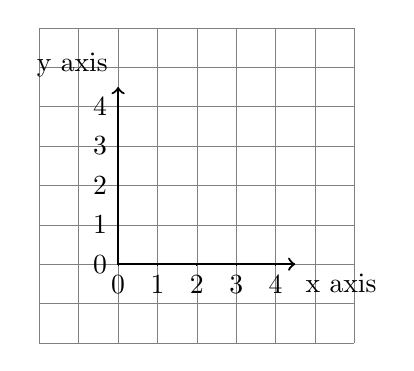
\begin{tikzpicture}[scale=.5]
\draw[step=1cm,gray,very thin] (-2,-2) grid (6,6);
\draw[thick,->] (0,0) -- (4.5,0) node[anchor=north west] {x axis};
\draw[thick,->] (0,0) -- (0,4.5) node[anchor=south east] {y axis};
\foreach \x in {0,1,2,3,4}
    \draw (\x cm,1pt) -- (\x cm,-1pt) node[anchor=north] {$\x$};
\foreach \y in {0,1,2,3,4}
    \draw (1pt,\y cm) -- (-1pt,\y cm) node[anchor=east] {$\y$};
\end{tikzpicture}
%%%%%%%%%%%%%%%%%%%%%%%%%%%%%%%%
\begin{verbatim}
%%%%%%xyplane%%%%%%
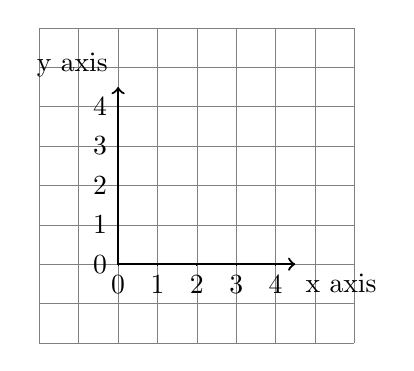
\begin{tikzpicture}[scale=.5]
\draw[step=1cm,gray,very thin] (-2,-2) grid (6,6);
\draw[thick,->] (0,0) -- (4.5,0) node[anchor=north west] {x axis};
\draw[thick,->] (0,0) -- (0,4.5) node[anchor=south east] {y axis};
\foreach \x in {0,1,2,3,4}
    \draw (\x cm,1pt) -- (\x cm,-1pt) node[anchor=north] {$\x$};
\foreach \y in {0,1,2,3,4}
    \draw (1pt,\y cm) -- (-1pt,\y cm) node[anchor=east] {$\y$};
\end{tikzpicture}
%%%%%%%%%%%%%%%%%%%%%%%%%%%%%%%%
\end{verbatim}
\hrule

%%%%%numberline with dots %%%%%%%%%%%%%%%%%%
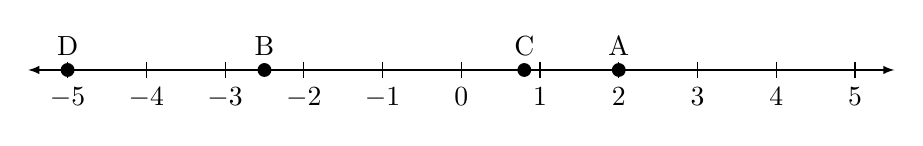
\begin{tikzpicture}[scale=1.0]
\begin{centering}
\draw[latex-latex] (-5.5,0) -- (5.5,0) ; %edit here for the axis
\foreach \x in  {-5,-4,-3,-2,-1,0,1,2,3,4,5} % edit here for the vertical lines
\draw[shift={(\x,0)},color=black] (0pt,3pt) -- (0pt,-3pt);
\foreach \x in {-5,-4,-3,-2,-1,0,1,2,3,4,5} % edit here for the numbers
\draw[shift={(\x,0)},color=black] (0pt,0pt) -- (0pt,-3pt) node[below] 
{$\x$};
%\draw[*-o] (0.92,0) -- (2.08,0);
\fill (-5,0)  circle[radius=2.5pt];
\node at (-5,.3) {D};
\fill (-2.5,0)  circle[radius=2.5pt];
\node at (-2.5,.3) {B};
\fill (0.8,0)  circle[radius=2.5pt];
\node at (0.8,.3) {C};
\fill (2,0)  circle[radius=2.5pt];
\node at (2,.3) {A};
%\draw (-2,0)  circle[radius=3pt]; 
%\draw[very thick] (0.92,0) -- (1.92,0);
\end{centering}
\end{tikzpicture}
%%%%%%%%%%%%%%%%%%%%%%%%%%%%%
\begin{verbatim}
%%%%%numberline with dots %%%%%%%%%%%%%%%%%%
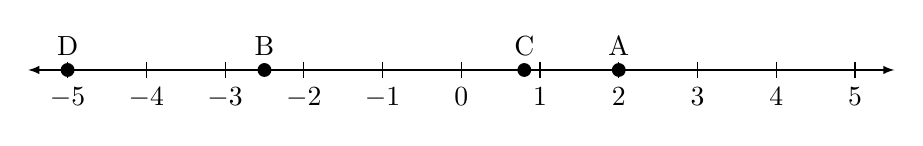
\begin{tikzpicture}[scale=1.0]
\begin{centering}
\draw[latex-latex] (-5.5,0) -- (5.5,0) ; %edit here for the axis
\foreach \x in  {-5,-4,-3,-2,-1,0,1,2,3,4,5} % edit here for the vertical lines
\draw[shift={(\x,0)},color=black] (0pt,3pt) -- (0pt,-3pt);
\foreach \x in {-5,-4,-3,-2,-1,0,1,2,3,4,5} % edit here for the numbers
\draw[shift={(\x,0)},color=black] (0pt,0pt) -- (0pt,-3pt) node[below] 
{$\x$};
%\draw[*-o] (0.92,0) -- (2.08,0);
\fill (-5,0)  circle[radius=2.5pt];
\node at (-5,.3) {D};
\fill (-2.5,0)  circle[radius=2.5pt];
\node at (-2.5,.3) {B};
\fill (0.8,0)  circle[radius=2.5pt];
\node at (0.8,.3) {C};
\fill (2,0)  circle[radius=2.5pt];
\node at (2,.3) {A};
%\draw (-2,0)  circle[radius=3pt]; 
%\draw[very thick] (0.92,0) -- (1.92,0);
\end{centering}
\end{tikzpicture}
%%%%%%%%%%%%%%%%%%%%%%%%%%%%%
\end{verbatim}\hrule

%%%%%%%%%%%%Quadrant I%%%%%%%%%%%%%%
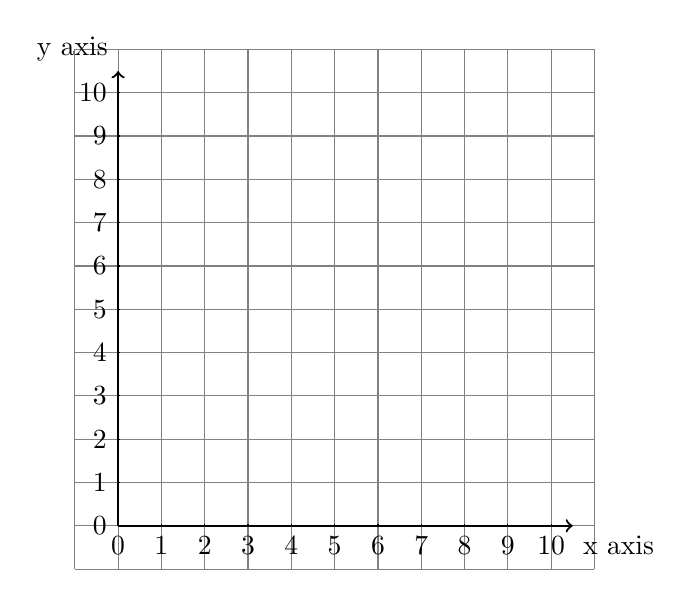
\begin{tikzpicture}[scale=.55]
%    \draw[gray] (0,0) grid (10,10);
\draw[step=1cm,gray, thin] (-1,-1) grid (11,11);
\draw[thick,->] (0,0) -- (10.5,0) node[anchor=north west] {x axis};
\draw[thick,->] (0,0) -- (0,10.5) node[anchor=south east] {y axis};
\foreach \x in {0,1,2,3,4,5,6,7,8,9,10}
    \draw (\x cm,1pt) -- (\x cm,-1pt) node[anchor=north] {$\x$};
\foreach \y in {0,1,2,3,4,5,6,7,8,9,10}
    \draw (1pt,\y cm) -- (-1pt,\y cm) node[anchor=east] {$\y$};
\end{tikzpicture}\\
%%%%%%%%%%%%%%%%%%%%%%%%%%%%%%%
\begin{verbatim}
%%%%%%%%%%%%Quadrant I%%%%%%%%%%%%%%
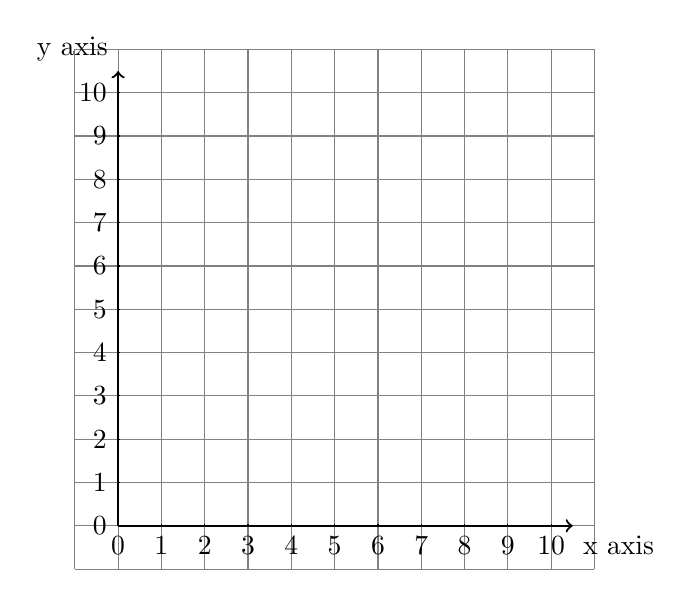
\begin{tikzpicture}[scale=.55]
%    \draw[gray] (0,0) grid (10,10);
\draw[step=1cm,gray, thin] (-1,-1) grid (11,11);
\draw[thick,->] (0,0) -- (10.5,0) node[anchor=north west] {x axis};
\draw[thick,->] (0,0) -- (0,10.5) node[anchor=south east] {y axis};
\foreach \x in {0,1,2,3,4,5,6,7,8,9,10}
    \draw (\x cm,1pt) -- (\x cm,-1pt) node[anchor=north] {$\x$};
\foreach \y in {0,1,2,3,4,5,6,7,8,9,10}
    \draw (1pt,\y cm) -- (-1pt,\y cm) node[anchor=east] {$\y$};
\end{tikzpicture}\\
%%%%%%%%%%%%%%%%%%%%%%%%%%%%%%%
\end{verbatim}\hrule

%%%%%%%%%%coordinate plane with points%%%%%%%%%
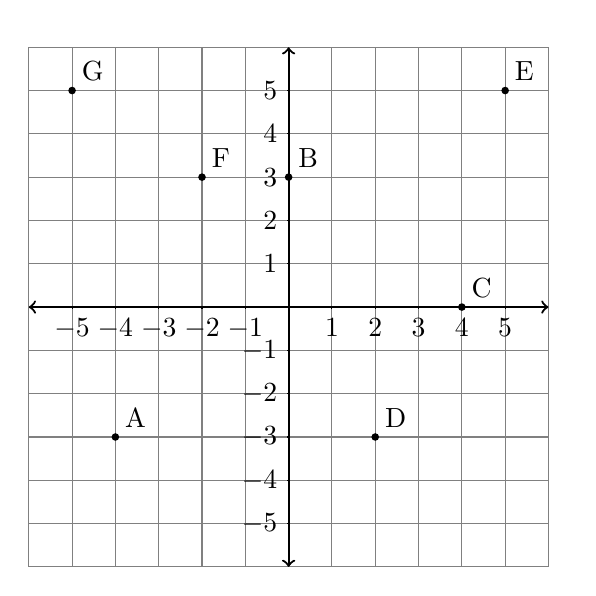
\begin{tikzpicture}[scale=.55]
%    \draw[gray] (0,0) grid (10,10);
\draw[step=1cm,gray, thin] (-6,-6) grid (6,6);
\draw[thick,<->] (-6,0) -- (6,0) node[anchor=north west] {};%{x};
\draw[thick,<->] (0,-6) -- (0,6) node[anchor=south east] {};%{y};
\foreach \x in {-5,-4,-3,-2,-1,1,2,3,4,5}
    \draw (\x cm,1pt) -- (\x cm,-1pt) node[anchor=north] {$\x$};
\foreach \y in {-5,-4,-3,-2,-1,1,2,3,4,5}
    \draw (1pt,\y cm) -- (-1pt,\y cm) node[anchor=east] {$\y$};
\fill (-4,-3)  circle[radius=2.5pt];
\fill (0,3)  circle[radius=2.5pt];
\fill (4,0)  circle[radius=2.5pt];
\fill (2,-3)  circle[radius=2.5pt];
\fill (5,5)  circle[radius=2.5pt];
\fill (-2,3)  circle[radius=2.5pt];
\fill (-5,5)  circle[radius=2.5pt];
\node[anchor=south west] at (-4,-3) {A};
\node[anchor=south west] at (0,3) {B};
\node[anchor=south west] at (4,0) {C};
\node[anchor=south west] at (2,-3) {D};
\node[anchor=south west] at (5,5) {E};
\node[anchor=south west] at (-2,3) {F};
\node[anchor=south west] at (-5,5) {G};
\end{tikzpicture}\\
%%%%%%%%%%%%%%%%%%%%%%%%%%
\begin{verbatim}
%%%%%%%%%%coordinate plane with points%%%%%%%%%
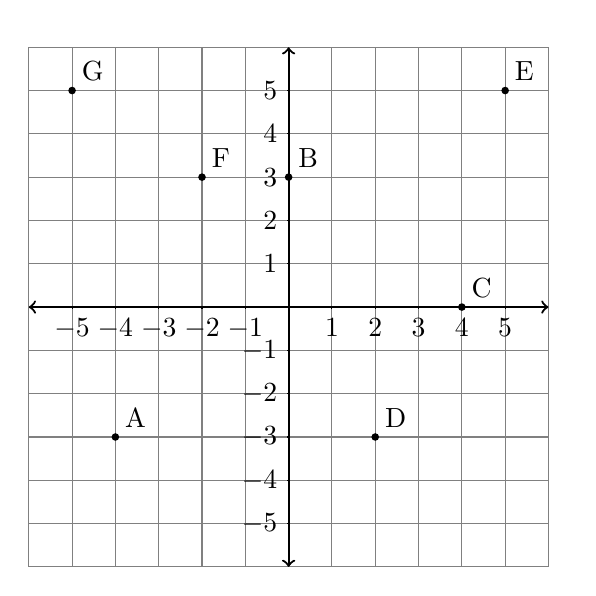
\begin{tikzpicture}[scale=.55]
%    \draw[gray] (0,0) grid (10,10);
\draw[step=1cm,gray, thin] (-6,-6) grid (6,6);
\draw[thick,<->] (-6,0) -- (6,0) node[anchor=north west] {};%{x};
\draw[thick,<->] (0,-6) -- (0,6) node[anchor=south east] {};%{y};
\foreach \x in {-5,-4,-3,-2,-1,1,2,3,4,5}
    \draw (\x cm,1pt) -- (\x cm,-1pt) node[anchor=north] {$\x$};
\foreach \y in {-5,-4,-3,-2,-1,1,2,3,4,5}
    \draw (1pt,\y cm) -- (-1pt,\y cm) node[anchor=east] {$\y$};
\fill (-4,-3)  circle[radius=2.5pt];
\fill (0,3)  circle[radius=2.5pt];
\fill (4,0)  circle[radius=2.5pt];
\fill (2,-3)  circle[radius=2.5pt];
\fill (5,5)  circle[radius=2.5pt];
\fill (-2,3)  circle[radius=2.5pt];
\fill (-5,5)  circle[radius=2.5pt];
\node[anchor=south west] at (-4,-3) {A};
\node[anchor=south west] at (0,3) {B};
\node[anchor=south west] at (4,0) {C};
\node[anchor=south west] at (2,-3) {D};
\node[anchor=south west] at (5,5) {E};
\node[anchor=south west] at (-2,3) {F};
\node[anchor=south west] at (-5,5) {G};
\end{tikzpicture}\\
%%%%%%%%%%%%%%%%%%%%%%%%%%
\end{verbatim}\hrule

%%%%%%%%%%coordinate plane with function%%%%%%%%%
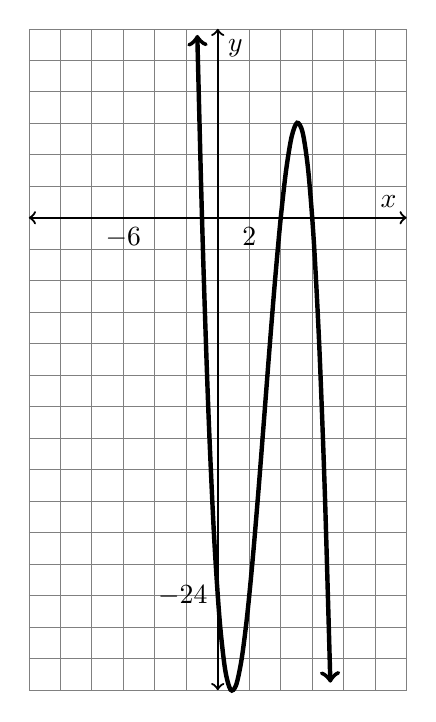
\begin{tikzpicture}[scale=.2]
\draw[style=help lines, ystep=2, xstep=2] (-12,-30) grid
  (12,12);
\draw[thick,<->] (-12,0) -- (12,0) node[anchor=south east] {$x$};
\draw[thick,<->] (0,-30) -- (0,12) node[anchor=north west] {$y$};
\foreach \x in {-6,2}
    \draw (\x cm,1pt) -- (\x cm,-1pt) node[anchor=north] {$\x$};
\foreach \y in {-24}
    \draw (1pt,\y cm) -- (-1pt,\y cm) node[anchor=east] {$\y$};
\draw[<->, ultra thick, domain=-1.3:7.15,smooth] plot (\x, {-1*(\x+1)*(\x-4)*(\x-6)});
\end{tikzpicture}\\
%%%%%%%%%%%%%%%%%%%%%%%%%%
\begin{verbatim}
%%%%%%%%%%coordinate plane with function%%%%%%%%%
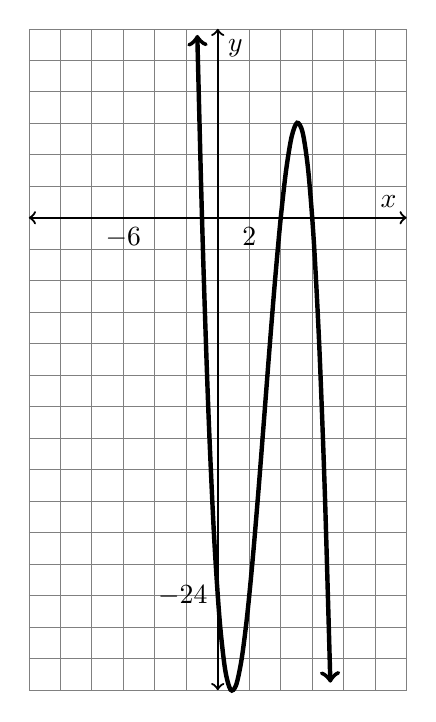
\begin{tikzpicture}[scale=.2]
\draw[style=help lines, ystep=2, xstep=2] (-12,-30) grid
  (12,12);
\draw[thick,<->] (-12,0) -- (12,0) node[anchor=south east] {$x$};
\draw[thick,<->] (0,-30) -- (0,12) node[anchor=north west] {$y$};
\foreach \x in {-6,2}
    \draw (\x cm,1pt) -- (\x cm,-1pt) node[anchor=north] {$\x$};
\foreach \y in {-24}
    \draw (1pt,\y cm) -- (-1pt,\y cm) node[anchor=east] {$\y$};
\draw[<->, ultra thick, domain=-1.3:7.15,smooth] plot (\x, {-1*(\x+1)*(\x-4)*(\x-6)});
\end{tikzpicture}\\
%%%%%%%%%%%%%%%%%%%%%%%%%%
\end{verbatim}\hrule

%%%%%%%%%%coordinate plane with function%%%%%%%%%
%\begin{tikzpicture}[scale=.2]
\begin{tikzpicture}[y=.05cm, x=.5cm]
\draw[style=help lines, ystep=10, xstep=1] (0,0) grid
  (10,60);
\draw[thick,-] (0,0) -- coordinate (x axis mid) (10,0);% node[anchor=south east] {$x$};
\draw[thick,-] (0,0) -- coordinate (y axis mid) (0,60);% node[anchor=north west] {$y$};
\foreach \x in {0,2,4,6,8,10}
    \draw (\x ,1pt) -- (\x ,-1pt) node[anchor=north] {$\x$};
\foreach \y in {0,20,40,60}
    \draw (1pt,\y ) -- (-1pt,\y ) node[anchor=east] {$\y$};
%\draw[<->, ultra thick, domain=-1.3:7.15,smooth] plot (\x, {-1*(\x+1)*(\x-4)*(\x-6)});
\draw[-, ultra thick, domain=-0:6,smooth] plot (\x, {10*\x}); %node[rotate=45,anchor=south east] {$Y$};
\node[rotate=45] at (4,45) {Yakov};
\node[rotate=0] at (7,35) {Demitri};
\draw[-, ultra thick, domain=-0:10,smooth] plot (\x, {5*\x+10}); %node[anchor=south east] {$D$};
\node[below=0.8cm] at (x axis mid) {Time (seconds)};
\node[rotate=90, above=0.8cm] at (y axis mid) {Distance (feet)};
\end{tikzpicture}\\
%%%%%%%%%%%%%%%%%%%%%%%%%%
\begin{verbatim}
%%%%%%%%%%coordinate plane with function%%%%%%%%%
%\begin{tikzpicture}[scale=.2]
\begin{tikzpicture}[y=.05cm, x=.5cm]
\draw[style=help lines, ystep=10, xstep=1] (0,0) grid
  (10,60);
\draw[thick,-] (0,0) -- coordinate (x axis mid) (10,0);% node[anchor=south east] {$x$};
\draw[thick,-] (0,0) -- coordinate (y axis mid) (0,60);% node[anchor=north west] {$y$};
\foreach \x in {0,2,4,6,8,10}
    \draw (\x ,1pt) -- (\x ,-1pt) node[anchor=north] {$\x$};
\foreach \y in {0,20,40,60}
    \draw (1pt,\y ) -- (-1pt,\y ) node[anchor=east] {$\y$};
%\draw[<->, ultra thick, domain=-1.3:7.15,smooth] plot (\x, {-1*(\x+1)*(\x-4)*(\x-6)});
\draw[-, ultra thick, domain=-0:6,smooth] plot (\x, {10*\x}); %node[rotate=45,anchor=south east] {$Y$};
\node[rotate=45] at (4,45) {Yakov};
\node[rotate=0] at (7,35) {Demitri};
\draw[-, ultra thick, domain=-0:10,smooth] plot (\x, {5*\x+10}); %node[anchor=south east] {$D$};
\node[below=0.8cm] at (x axis mid) {Time (seconds)};
\node[rotate=90, above=0.8cm] at (y axis mid) {Distance (feet)};
\end{tikzpicture}\\
%%%%%%%%%%%%%%%%%%%%%%%%%%
\end{verbatim}\hrule

%%%%%%%%%%coordinate plane with function%%%%%%%%%
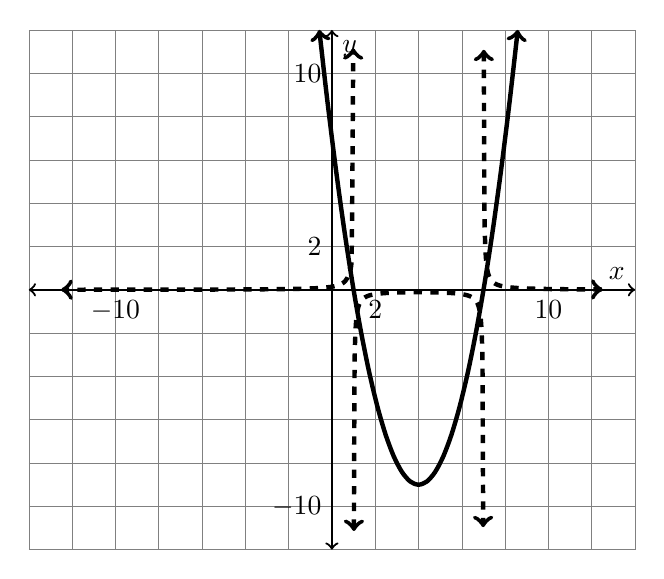
\begin{tikzpicture}[scale=.275]
\draw[style=help lines, ystep=2, xstep=2] (-14,-12) grid
  (14,12);
\draw[thick,<->] (-14,0) -- (14,0) node[anchor=south east] {$x$};
\draw[thick,<->] (0,-12) -- (0,12) node[anchor=north west] {$y$};
\foreach \x in {-10,2,10}
    \draw (\x cm,1pt) -- (\x cm,-1pt) node[anchor=north] {$\x$};
\foreach \y in {-10,2,10}
    \draw (1pt,\y cm) -- (-1pt,\y cm) node[anchor=east] {$\y$};
\draw[<->, ultra thick, domain=-.583:8.583,smooth] plot (\x, {\x*\x-8*\x+7});
\draw[dashed,<->, ultra thick, domain=-12.5:.986,smooth,samples=200] plot (\x, {1/(\x*\x-8*\x+7)});
\draw[dashed,<->, ultra thick, domain=1.015:6.987,smooth,samples=200] plot (\x, {1/(\x*\x-8*\x+7)});
\draw[dashed,<->, ultra thick, domain=7.015:12.5,smooth,samples=200] plot (\x, {1/(\x*\x-8*\x+7)});
\end{tikzpicture}
%%%%%%%%%%%%%%%%%%%%%%%%%%

\begin{verbatim}
%%%%%%%%%%coordinate plane with function%%%%%%%%%
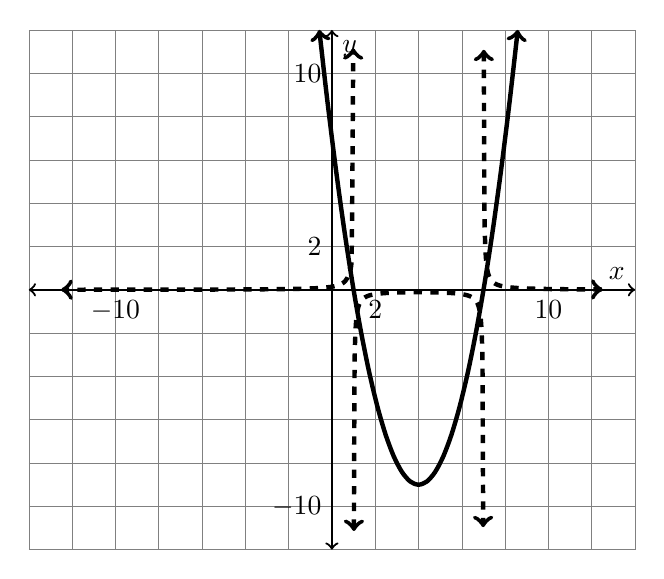
\begin{tikzpicture}[scale=.275]
\draw[style=help lines, ystep=2, xstep=2] (-14,-12) grid
  (14,12);
\draw[thick,<->] (-14,0) -- (14,0) node[anchor=south east] {$x$};
\draw[thick,<->] (0,-12) -- (0,12) node[anchor=north west] {$y$};
\foreach \x in {-10,2,10}
    \draw (\x cm,1pt) -- (\x cm,-1pt) node[anchor=north] {$\x$};
\foreach \y in {-10,2,10}
    \draw (1pt,\y cm) -- (-1pt,\y cm) node[anchor=east] {$\y$};
\draw[<->, ultra thick, domain=-.583:8.583,smooth] plot (\x, {\x*\x-8*\x+7});
\draw[dashed,<->, ultra thick, domain=-12.5:.986,smooth,samples=200] plot (\x, {1/(\x*\x-8*\x+7)});
\draw[dashed,<->, ultra thick, domain=1.015:6.987,smooth,samples=200] plot (\x, {1/(\x*\x-8*\x+7)});
\draw[dashed,<->, ultra thick, domain=7.015:12.5,smooth,samples=200] plot (\x, {1/(\x*\x-8*\x+7)});
\end{tikzpicture}
%%%%%%%%%%%%%%%%%%%%%%%%%%
\end{verbatim}
\hrule














%%%%%%%%%angle%%%%%%%%%%%%%%%%%
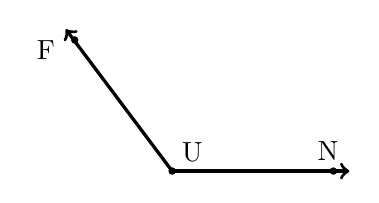
\begin{tikzpicture}[scale=.45]
%    \draw[gray] (0,0) grid (10,10);
\draw[ very thick,->] (4,1) -- (1,5) node[anchor=north east] {F};
\fill (1.25,4.7)  circle[radius=3pt];
\draw[very thick,->] (4,1) -- (9,1) node[anchor=south east] {N};
\fill (8.55,1)  circle[radius=3pt];
\fill (4,1)  circle[radius=3pt] node[anchor=south west]{U};
\end{tikzpicture}\\
%%%%%%%%%%%%%%%%%%%%%%%%%%%%
\begin{verbatim}
%%%%%%%%%angle%%%%%%%%%%%%%%%%%
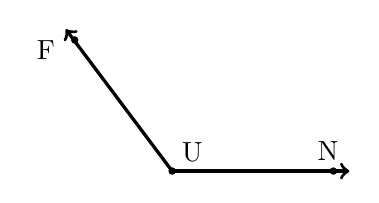
\begin{tikzpicture}[scale=.45]
%    \draw[gray] (0,0) grid (10,10);
\draw[ very thick,->] (4,1) -- (1,5) node[anchor=north east] {F};
\fill (1.25,4.7)  circle[radius=3pt];
\draw[very thick,->] (4,1) -- (9,1) node[anchor=south east] {N};
\fill (8.55,1)  circle[radius=3pt];
\fill (4,1)  circle[radius=3pt] node[anchor=south west]{U};
\end{tikzpicture}\\
%%%%%%%%%%%%%%%%%%%%%%%%%%%%
\end{verbatim}\hrule

%%%%%%%%%%%parallel lines w/transversal%%%%%%%%%
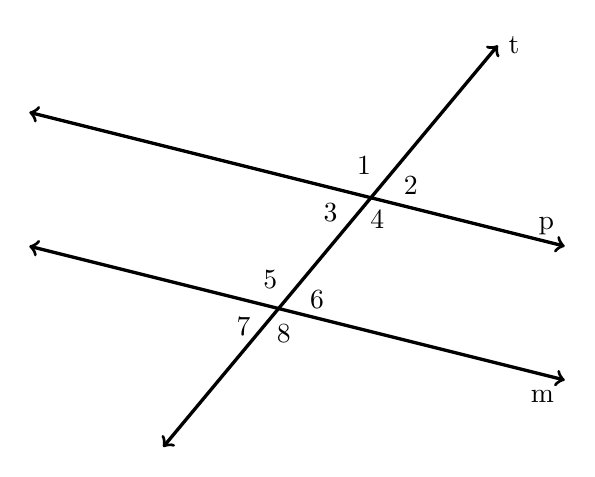
\begin{tikzpicture}[scale=.85]
%\draw[gray] (0,0) grid (10,10);
\draw[ very thick,<->] (1,4) -- (9,2) node[anchor=north east] {m};
%\fill (1.25,4.7)  circle[radius=3pt];
\draw[very thick,<->] (1,6) -- (9,4) node[anchor=south east] {p};
%\fill (8.55,1)  circle[radius=3pt];
\draw[ very thick,<->] (3,1) -- (8,7) node[anchor=west] {t};
%\fill (4,1)  circle[radius=3pt] node[anchor=south west]{U};
\node at (6,5.2) {1};
\node at (6.7,4.9) {2};
\node at (5.5,4.5) {3};
\node at (6.2,4.4) {4};
\node at (4.6,3.5) {5};
\node at (5.3,3.2) {6};
\node at (4.2,2.8) {7};
\node at (4.8,2.7) {8};
\end{tikzpicture}\\
%%%%%%%%%%%%%%%%%%%%%%%%%%%%%%%
\begin{verbatim}
%%%%%%%%%%%parallel lines w/transversal%%%%%%%%%
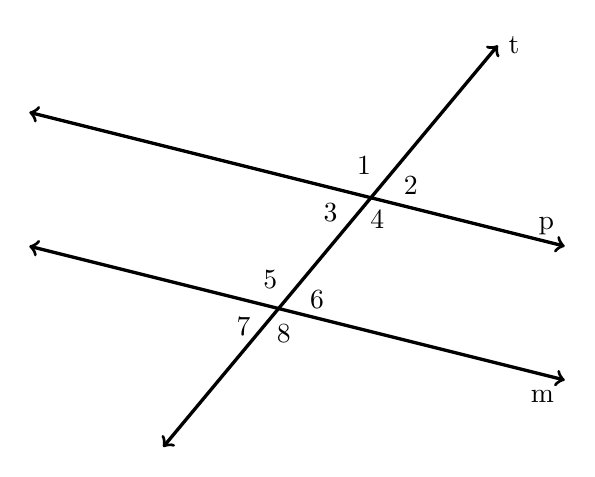
\begin{tikzpicture}[scale=.85]
%\draw[gray] (0,0) grid (10,10);
\draw[ very thick,<->] (1,4) -- (9,2) node[anchor=north east] {m};
%\fill (1.25,4.7)  circle[radius=3pt];
\draw[very thick,<->] (1,6) -- (9,4) node[anchor=south east] {p};
%\fill (8.55,1)  circle[radius=3pt];
\draw[ very thick,<->] (3,1) -- (8,7) node[anchor=west] {t};
%\fill (4,1)  circle[radius=3pt] node[anchor=south west]{U};
\node at (6,5.2) {1};
\node at (6.7,4.9) {2};
\node at (5.5,4.5) {3};
\node at (6.2,4.4) {4};
\node at (4.6,3.5) {5};
\node at (5.3,3.2) {6};
\node at (4.2,2.8) {7};
\node at (4.8,2.7) {8};
\end{tikzpicture}\\
%%%%%%%%%%%%%%%%%%%%%%%%%%%%%%%
\end{verbatim}\hrule

%%%%%%%%%%%TRIG SCALE GRAPH%%%%%%%%%%%
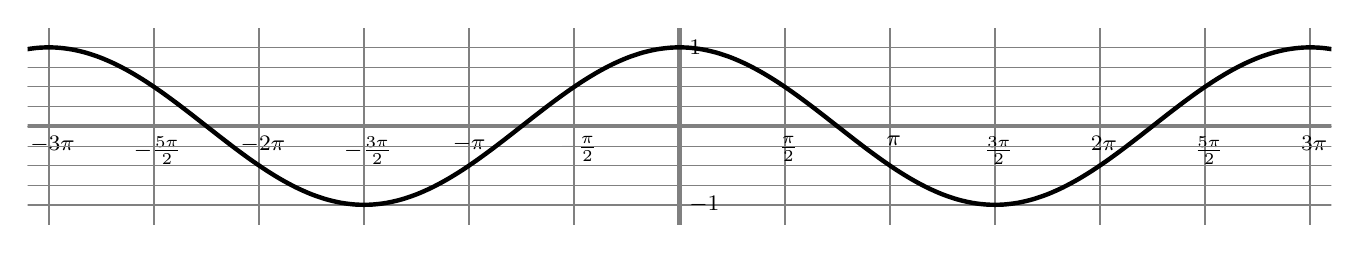
\begin{tikzpicture}[xscale=.85, yscale=1]
    \clip (-3.1*pi,-1.25) rectangle (3.1*pi,1.25);
    \draw[ultra thick, gray] (-4.25*pi,0) -- (4.25*pi,0);
    \draw[ultra thick, gray] (0,-1.25) -- (0,1.25);
    \foreach \x/\xtext in {
                        -4*pi / $-4\pi$,
                        -3.5*pi / $-\frac{7\pi}{2}$,
                        -3*pi / $-3\pi $,
                        -2.5*pi / $-\frac{5\pi}{2} $,
                        -2*pi / $-2\pi $,
                        -1.5*pi / $-\frac{3\pi}{2} $,
                        -pi /$-\pi$,
                        -0.5*pi / $-\frac{\pi}{2} $,
                        0 / {},
                        0.5*pi / $\frac{\pi}{2} $,
                        pi / $\pi$,
                        1.5*pi / $\frac{3\pi}{2} $,
                        2*pi / $2\pi $,
                        2.5*pi / $\frac{5\pi}{2} $,
                        3*pi / $3\pi $,
                        3.5*pi / $\frac{7\pi}{2}$,
                        4*pi / $4\pi$
                        }
    {
        \draw[thick, gray] (\x,-1.25) -- node [black, below] {\footnotesize{\xtext}} (\x,1.25); 
        %\foreach \p in {6,4,3} {
            %\draw[thin, gray] (\x + 3.1416/\p,-1.25) -- (\x + 3.1416/\p,1.25); 
        %}
    };
    \foreach \y in {-1,-0.75,...,1}
    {
        \draw[very thin, gray] (-10,\y) -- (10,\y);
    };
    \foreach \y in {-1,-0.5,...,1}
    {
        \draw[thin, gray] (-10,\y) -- (10,\y);
    };
    \draw (0,1) node[right]{\footnotesize{$1 $}};
    \draw (0,-1) node[right]{\footnotesize{$-1 $}};
    %\draw [rootthreeovertwo] (-10,0.866) -- (10,0.866);
    %\draw [rootthreeovertwo] (-10,-0.866) -- (10,-0.866);  
    %\draw [roottwovertwo] (-10,.7071) --(10,.7071);
    %\draw [roottwovertwo] (-10,-.7071) --(10,-.7071);
    %#1
\draw[ultra thick, smooth,domain=-10:10, samples=90]    plot (\x,{cos((2/3)*\x r)});
\end{tikzpicture}
%%%%%%%%%%%%%%%%%%%%%%%%%%%%%%%%%%%%%
\begin{verbatim}
%%%%%%%%%%%TRIG SCALE GRAPH%%%%%%%%%%%
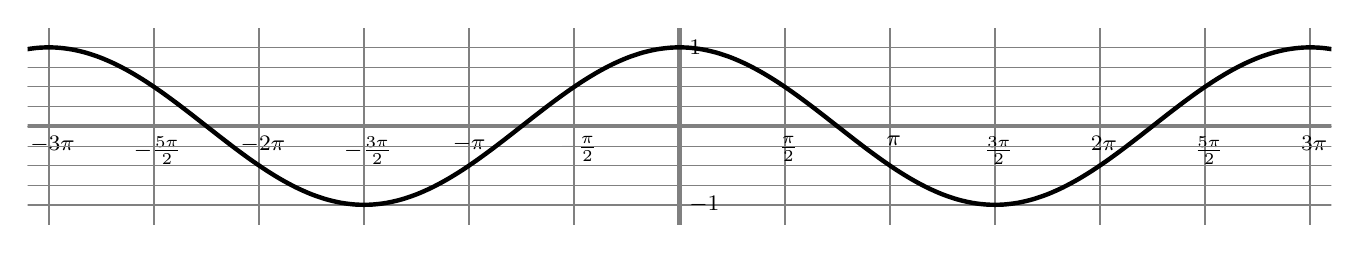
\begin{tikzpicture}[xscale=.85, yscale=1]
    \clip (-3.1*pi,-1.25) rectangle (3.1*pi,1.25);
    \draw[ultra thick, gray] (-4.25*pi,0) -- (4.25*pi,0);
    \draw[ultra thick, gray] (0,-1.25) -- (0,1.25);
    \foreach \x/\xtext in {
                        -4*pi / $-4\pi$,
                        -3.5*pi / $-\frac{7\pi}{2}$,
                        -3*pi / $-3\pi $,
                        -2.5*pi / $-\frac{5\pi}{2} $,
                        -2*pi / $-2\pi $,
                        -1.5*pi / $-\frac{3\pi}{2} $,
                        -pi /$-\pi$,
                        -0.5*pi / $-\frac{\pi}{2} $,
                        0 / {},
                        0.5*pi / $\frac{\pi}{2} $,
                        pi / $\pi$,
                        1.5*pi / $\frac{3\pi}{2} $,
                        2*pi / $2\pi $,
                        2.5*pi / $\frac{5\pi}{2} $,
                        3*pi / $3\pi $,
                        3.5*pi / $\frac{7\pi}{2}$,
                        4*pi / $4\pi$
                        }
    {
        \draw[thick, gray] (\x,-1.25) -- node [black, below] {\footnotesize{\xtext}} (\x,1.25); 
        %\foreach \p in {6,4,3} {
            %\draw[thin, gray] (\x + 3.1416/\p,-1.25) -- (\x + 3.1416/\p,1.25); 
        %}
    };
    \foreach \y in {-1,-0.75,...,1}
    {
        \draw[very thin, gray] (-10,\y) -- (10,\y);
    };
    \foreach \y in {-1,-0.5,...,1}
    {
        \draw[thin, gray] (-10,\y) -- (10,\y);
    };
    \draw (0,1) node[right]{\footnotesize{$1 $}};
    \draw (0,-1) node[right]{\footnotesize{$-1 $}};
    %\draw [rootthreeovertwo] (-10,0.866) -- (10,0.866);
    %\draw [rootthreeovertwo] (-10,-0.866) -- (10,-0.866);  
    %\draw [roottwovertwo] (-10,.7071) --(10,.7071);
    %\draw [roottwovertwo] (-10,-.7071) --(10,-.7071);
    %#1
\draw[ultra thick, smooth,domain=-10:10, samples=90]    plot (\x,{cos((2/3)*\x r)});
\end{tikzpicture}
%%%%%%%%%%%%%%%%%%%%%%%%%%%%%%%%%%%%%
\end{verbatim}\hrule
\newpage
\begin{question}[class=easy]
Let $d=t^{2}$ denote the distance $d$ (in feet) that Jerry has walked in $t$ seconds. The graph of this function is shown below.
\begin{figure}[h]
	   \begin{minipage}[c]{3cm}
	%%%%%%%%%%coordinate plane with function%%%%%%%%%
	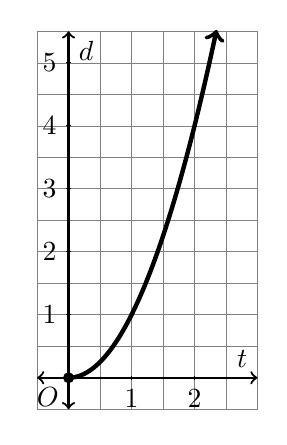
\begin{tikzpicture}[scale=.8]
	\draw[style=help lines, ystep=.5, xstep=.5] (-.5,-.5) grid (3,5.5);
	\draw[thick,<->] (-.5,0) -- (3,0) node[anchor=south east] {$t$};
	\draw[thick,<->] (0,-.5) -- (0,5.5) node[anchor=north west] {$d$};
	\foreach \x in {1,2}
	   \draw (\x ,1pt) -- (\x ,-1pt) node[anchor=north] {$\x$};
	\foreach \y in {1,2,3,4,5}
	    \draw (1pt,\y ) -- (-1pt,\y ) node[anchor=east] {$\y$};
	\draw[->, ultra thick, domain=0:2.35,smooth] plot (\x, {(\x)*(\x)});
	\fill (0,0)  circle[radius=2.5pt];
	\node[anchor=north east] at (0,0) {$O$};
	\end{tikzpicture}
	%%%%%%%%%%%%%%%%%%%%%%%%%% 
	   \end{minipage}%
	   \begin{minipage}[c]{4cm}
	\begin{enumerate}
	\item Determine his average speed between $t=1$ and $t=2$. 
	\item Determine his average speed between $t=1$ and $t=1.1$.
	\item Determine his average speed between $t=1$ and $t=1.01$.
	\item Determine his instantaneous speed at $t=1$.
	\end{enumerate}
	   \end{minipage}
	%   \caption{Your image}
	\end{figure}
\end{question}
\begin{solution}
\begin{enumerate}
\item 3 ft/s
\item 2.1 ft/s
\item 2.01 f/s
\item 2 ft/s
\end{enumerate}�
 \cite[p.197]{Project2008}
\end{solution}

\begin{verbatim}
\begin{question}[class=easy]
Let $d=t^{2}$ denote the distance $d$ (in feet) that Jerry has walked in $t$ seconds. The graph of this function is shown below.
\begin{figure}[h]%play with options: h, t, !, b, p
	   \begin{minipage}[c]{3cm}
	%%%%%%%%%%coordinate plane with function%%%%%%%%%
	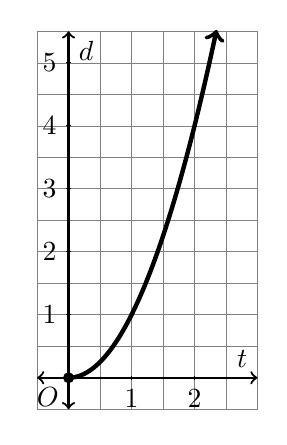
\begin{tikzpicture}[scale=.8]
	\draw[style=help lines, ystep=.5, xstep=.5] (-.5,-.5) grid (3,5.5);
	\draw[thick,<->] (-.5,0) -- (3,0) node[anchor=south east] {$t$};
	\draw[thick,<->] (0,-.5) -- (0,5.5) node[anchor=north west] {$d$};
	\foreach \x in {1,2}
	   \draw (\x ,1pt) -- (\x ,-1pt) node[anchor=north] {$\x$};
	\foreach \y in {1,2,3,4,5}
	    \draw (1pt,\y ) -- (-1pt,\y ) node[anchor=east] {$\y$};
	\draw[->, ultra thick, domain=0:2.35,smooth] plot (\x, {(\x)*(\x)});
	\fill (0,0)  circle[radius=2.5pt];
	\node[anchor=north east] at (0,0) {$O$};
	\end{tikzpicture}
	%%%%%%%%%%%%%%%%%%%%%%%%%% 
	   \end{minipage}%
	   \begin{minipage}[c]{4cm}
	\begin{enumerate}
	\item Determine his average speed between $t=1$ and $t=2$. 
	\item Determine his average speed between $t=1$ and $t=1.1$.
	\item Determine his average speed between $t=1$ and $t=1.01$.
	\item Determine his instantaneous speed at $t=1$.
	\end{enumerate}
	   \end{minipage}
	%   \caption{Your image}
	\end{figure}
\end{question}
\begin{solution}
\begin{enumerate}
\item 3 ft/s
\item 2.1 ft/s
\item 2.01 f/s
\item 2 ft/s
\end{enumerate}�
 \cite[p.197]{Project2008}
\end{solution}
\end{verbatim}\hrule

	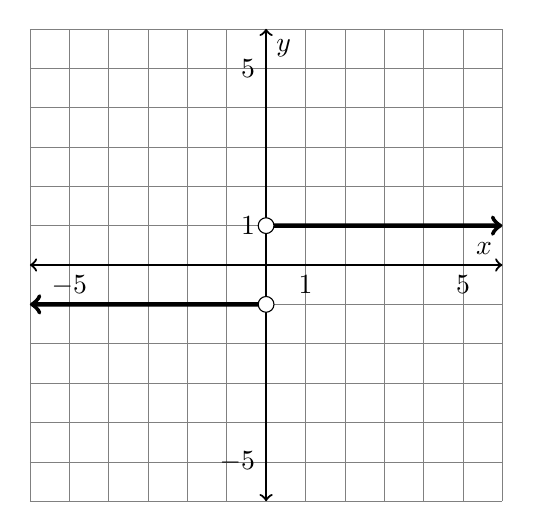
\begin{tikzpicture}[scale=.5]
	\draw[style=help lines, ystep=1, xstep=1] (-6,-6) grid
	  (6,6);
	\draw[thick,<->] (-6,0) -- (6,0) node[anchor=south east] {$x$};
	\draw[thick,<->] (0,-6) -- (0,6) node[anchor=north west] {$y$};
	\foreach \x in {-5,1,5}
	    \draw (\x cm,1pt) -- (\x cm,-1pt) node[anchor=north] {$\x$};
	\foreach \y in {-5,1,5}
	    \draw (1pt,\y cm) -- (-1pt,\y cm) node[anchor=east] {$\y$};
	\draw[<-, ultra thick, domain=-6:-.001,smooth] plot (\x, {abs(\x)/\x});
	\draw[->, ultra thick, domain=.001:6,smooth] plot (\x, {abs(\x)/\x});
	\draw[fill=white] (0,1) circle (.2cm);
		\draw[fill=white] (0,-1) circle (.2cm);
	\end{tikzpicture}

\begin{verbatim}
	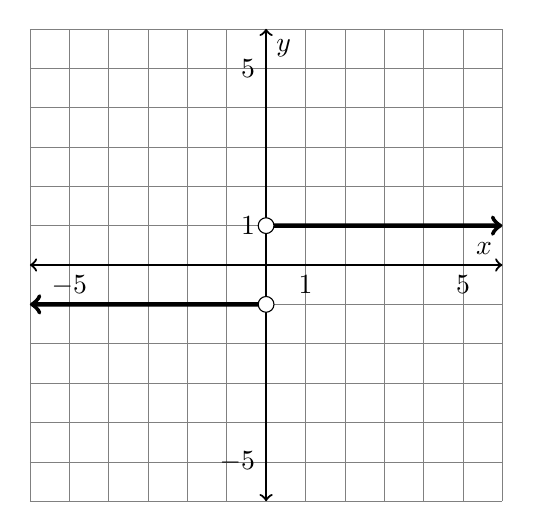
\begin{tikzpicture}[scale=.5]
	\draw[style=help lines, ystep=1, xstep=1] (-6,-6) grid
	  (6,6);
	\draw[thick,<->] (-6,0) -- (6,0) node[anchor=south east] {$x$};
	\draw[thick,<->] (0,-6) -- (0,6) node[anchor=north west] {$y$};
	\foreach \x in {-5,1,5}
	    \draw (\x cm,1pt) -- (\x cm,-1pt) node[anchor=north] {$\x$};
	\foreach \y in {-5,1,5}
	    \draw (1pt,\y cm) -- (-1pt,\y cm) node[anchor=east] {$\y$};
	\draw[<-, ultra thick, domain=-6:-.001,smooth] plot (\x, {abs(\x)/\x});
	\draw[->, ultra thick, domain=.001:6,smooth] plot (\x, {abs(\x)/\x});
	\draw[fill=white] (0,1) circle (.2cm);
		\draw[fill=white] (0,-1) circle (.2cm);
	\end{tikzpicture}
\end{verbatim} \hrule


\begin{table}[ht] 
	%\caption{Nonlinear Model Results} % title of Table 
	\centering % used for centering table 
	\begin{tabular}{c c} % centered columns (2 columns) 
	\hline %inserts double horizontal lines 
	$x$& $k(x)$ \\ [0.5ex] % inserts table 
	%heading 
	\hline\hline % inserts single horizontal line 
	0 & 2  \\ % inserting body of the table 
	1 & \framebox[1.1\width]{\rule{0pt}{.1in}\quad\quad} \par  \\ [1ex]
	2 & \framebox[1.1\width]{\rule{0pt}{.1in}\quad\quad} \par  \\ [1ex]
	3 & \framebox[1.1\width]{\rule{0pt}{.1in}\quad\quad} \par  \\ [1ex]
	4 & \framebox[1.1\width]{\rule{0pt}{.1in}\quad\quad} \par   \\ [1ex] % [1ex] adds vertical space 
	\hline %inserts single line 
	\end{tabular} 
	%\label{table:nonlin} % is used to refer this table in the text 
	\end{table} 

\begin{verbatim}
	%%%%%%%%%Table%%%%%%%%%%%%%%
	\begin{table}[ht] 
	%\caption{Nonlinear Model Results} % title of Table 
	\centering % used for centering table 
	\begin{tabular}{c c} % centered columns (2 columns) 
	\hline %inserts double horizontal lines 
	$x$& $k(x)$ \\ [0.5ex] % inserts table 
	%heading 
	\hline\hline % inserts single horizontal line 
	0 & 2  \\ % inserting body of the table 
	1 & \framebox[1.1\width]{\rule{0pt}{.1in}\quad\quad} \par  \\ [1ex]
	2 & \framebox[1.1\width]{\rule{0pt}{.1in}\quad\quad} \par  \\ [1ex]
	3 & \framebox[1.1\width]{\rule{0pt}{.1in}\quad\quad} \par  \\ [1ex]
	4 & \framebox[1.1\width]{\rule{0pt}{.1in}\quad\quad} \par   \\ [1ex] % [1ex] adds vertical space 
	\hline %inserts single line 
	\end{tabular} 
	%\label{table:nonlin} % is used to refer this table in the text 
	\end{table} 
\end{verbatim}�
\hrule

%%%%%%%%%%%%%SAWTOOTH%%%%%%%%%%%%
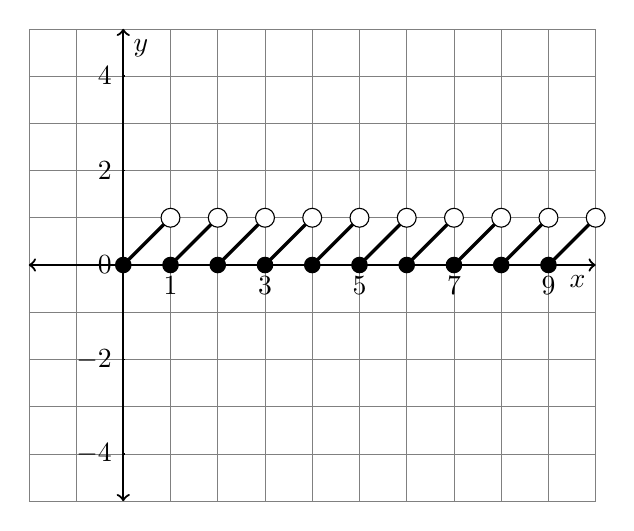
\begin{tikzpicture}[scale=.6]
	\draw[style=help lines, ystep=1, xstep=1] (-2,-5) grid
	  (10,5);
	\draw[thick,<->] (-2,0) -- (10,0) node[anchor=north east] {$x$};
	\draw[thick,<->] (0,-5) -- (0,5) node[anchor=north west] {$y$};
	\foreach \x in {1,3,5,7,9}
	    \draw (\x cm,1pt) -- (\x cm,-1pt) node[anchor=north] {$\x$};
	\foreach \y in {-4,-2,0,2,4}
	\draw (1pt,\y cm) -- (-1pt,\y cm) node[anchor=east] {$\y$};
	\foreach \a in {0,1,...,9}
		\draw[very thick] plot[domain=\a:\a+1] (\x,{\x-floor(\x)}); %node[right] {\footnotesize $[x]$};
	\foreach \b in {0,1,...,9}
		\fill (\b,0) circle[radius=5pt];	
	\foreach \c in {0,1,...,9}
		\draw[fill=white] (\c+1,1) circle (.2cm);
\end{tikzpicture}\\
%%%%%%%%%%%%%%%%%%%%%%%%%%%%%%%%%
\begin{verbatim}
%%%%%%%%%%%%%SAWTOOTH%%%%%%%%%%%%
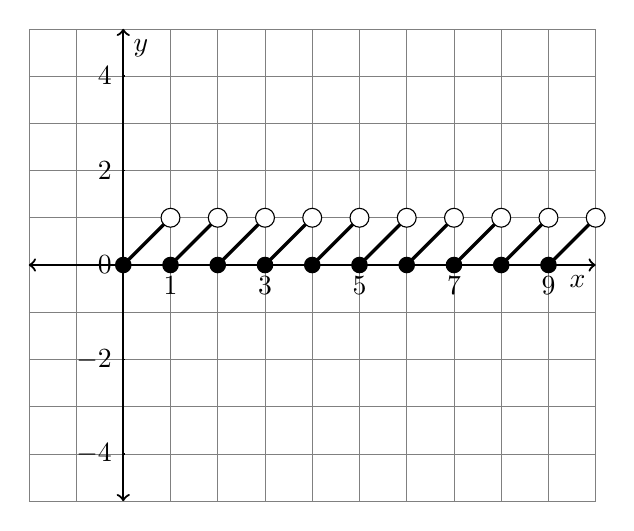
\begin{tikzpicture}[scale=.6]
	\draw[style=help lines, ystep=1, xstep=1] (-2,-5) grid
	  (10,5);
	\draw[thick,<->] (-2,0) -- (10,0) node[anchor=north east] {$x$};
	\draw[thick,<->] (0,-5) -- (0,5) node[anchor=north west] {$y$};
	\foreach \x in {1,3,5,7,9}
	    \draw (\x cm,1pt) -- (\x cm,-1pt) node[anchor=north] {$\x$};
	\foreach \y in {-4,-2,0,2,4}
	\draw (1pt,\y cm) -- (-1pt,\y cm) node[anchor=east] {$\y$};
	\foreach \a in {0,1,...,9}
		\draw[very thick] plot[domain=\a:\a+1] (\x,{\x-floor(\x)}); %node[right] {\footnotesize $[x]$};
	\foreach \b in {0,1,...,9}
		\fill (\b,0) circle[radius=5pt];	
	\foreach \c in {0,1,...,9}
		\draw[fill=white] (\c+1,1) circle (.2cm);
\end{tikzpicture}\\
%%%%%%%%%%%%%%%%%%%%%%%%%%%%%%%%%
\end{verbatim}
\hrule

%%%%%%%%%%Exponential%%%%%%%%%%%%%%%%%%
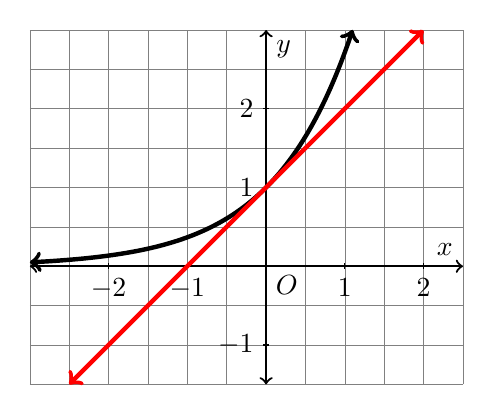
\begin{tikzpicture}[scale=1]
	\draw[style=help lines, ystep=.5, xstep=.5] (-3,-1.5) grid (2.5,3);
	\draw[thick,<->] (-3,0) -- (2.5,0) node[anchor=south east] {$x$};
	\draw[thick,<->] (0,-1.5) -- (0,3) node[anchor=north west] {$y$};
	\foreach \x in {-2, -1, 1, 2}
	    \draw (\x cm,1pt) -- (\x cm,-1pt) node[anchor=north] {$\x$};
	\foreach \y in {-1, 1, 2}
	    \draw (1pt,\y cm) -- (-1pt,\y cm) node[anchor=east] {$\y$};
	\node[anchor=north west] at (0,0) {$O$};
	\draw[<->, ultra thick, domain=-3:1.1,smooth,samples=200] plot (\x, {e^\x});
	\draw[<->, red,ultra thick, domain=-2.5:2,smooth,samples=200] plot (\x, {\x+1});
	\end{tikzpicture}
%%%%%%%%%%%%%%%%%%%%%%%%%%%%%%%%%%%
\begin{verbatim}
{\bf NOTE} plot (\x, {e^\x}) not plot (\x, {e^{\x}})
%%%%%%%%%%Exponential%%%%%%%%%%%%%%%%%%
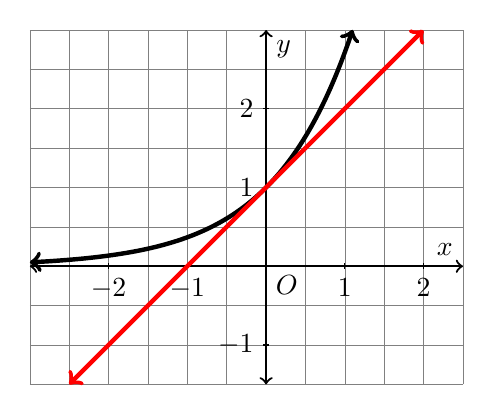
\begin{tikzpicture}[scale=1]
	\draw[style=help lines, ystep=.5, xstep=.5] (-3,-1.5) grid (2.5,3);
	\draw[thick,<->] (-3,0) -- (2.5,0) node[anchor=south east] {$x$};
	\draw[thick,<->] (0,-1.5) -- (0,3) node[anchor=north west] {$y$};
	\foreach \x in {-2, -1, 1, 2}
	    \draw (\x cm,1pt) -- (\x cm,-1pt) node[anchor=north] {$\x$};
	\foreach \y in {-1, 1, 2}
	    \draw (1pt,\y cm) -- (-1pt,\y cm) node[anchor=east] {$\y$};
	\node[anchor=north west] at (0,0) {$O$};
	\draw[<->, ultra thick, domain=-3:1.1,smooth,samples=200] plot (\x, {e^\x});
	\draw[<->, red,ultra thick, domain=-2.5:2,smooth,samples=200] plot (\x, {\x+1});
	\end{tikzpicture}
%%%%%%%%%%%%%%%%%%%%%%%%%%%%%%%%%%%
\end{verbatim}�
\hrule

%%%%%%%%%%%%%LOG%%%%%%%%%%%%%%%%%%%%
	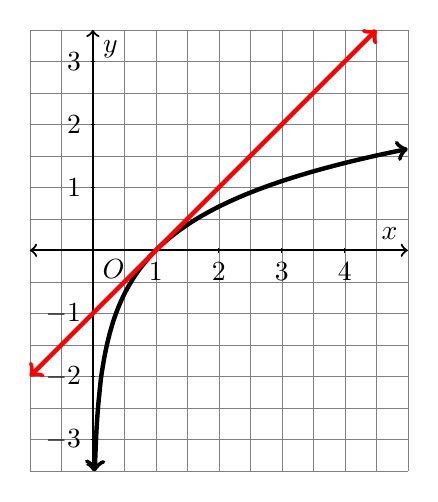
\begin{tikzpicture}[scale=.8]
	\draw[style=help lines, ystep=.5, xstep=.5] (-1,-3.5) grid (5,3.5);
	\draw[thick,<->] (-1,0) -- (5,0) node[anchor=south east] {$x$};
	\draw[thick,<->] (0,-3.5) -- (0,3.5) node[anchor=north west] {$y$};
	\foreach \x in {1, 2,3,4}
	    \draw (\x cm,1pt) -- (\x cm,-1pt) node[anchor=north] {$\x$};
	\foreach \y in {-3,-2,-1,1,2,3}
	    \draw (1pt,\y cm) -- (-1pt,\y cm) node[anchor=east] {$\y$};
	\node[anchor=north west] at (0,0) {$O$};
	\draw[<->, ultra thick, domain=.03:5,smooth,samples=200] plot (\x, {ln{\x}});
%	\draw[<->, ultra thick, domain=.03:5,smooth,samples=200] plot (\x, {log2{\x}});
	\draw[<->, red,ultra thick, domain=-1:4.5,smooth,samples=200] plot (\x, {\x-1});
	\end{tikzpicture}\\
%%%%%%%%%%%%%%%%%%%%%%%%%%%%%%%%%%%%%
\begin{verbatim}
%%%%%%%%%%%%%LOG%%%%%%%%%%%%%%%%%%%%
	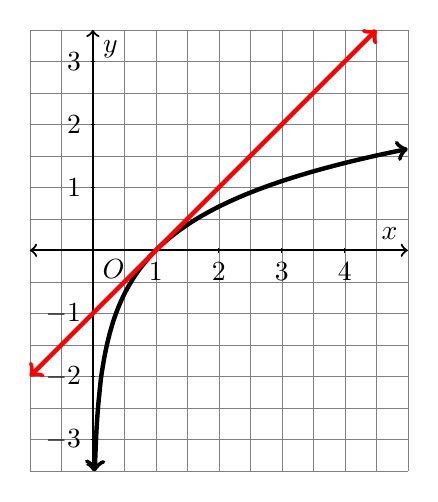
\begin{tikzpicture}[scale=.8]
	\draw[style=help lines, ystep=.5, xstep=.5] (-1,-3.5) grid (5,3.5);
	\draw[thick,<->] (-1,0) -- (5,0) node[anchor=south east] {$x$};
	\draw[thick,<->] (0,-3.5) -- (0,3.5) node[anchor=north west] {$y$};
	\foreach \x in {1, 2,3,4}
	    \draw (\x cm,1pt) -- (\x cm,-1pt) node[anchor=north] {$\x$};
	\foreach \y in {-3,-2,-1,1,2,3}
	    \draw (1pt,\y cm) -- (-1pt,\y cm) node[anchor=east] {$\y$};
	\node[anchor=north west] at (0,0) {$O$};
	\draw[<->, ultra thick, domain=.03:5,smooth,samples=200] plot (\x, {ln{\x}});
%	\draw[<->, ultra thick, domain=.03:5,smooth,samples=200] plot (\x, {log2{\x}});
	\draw[<->, red,ultra thick, domain=-1:4.5,smooth,samples=200] plot (\x, {\x-1});
	\end{tikzpicture}\\
%%%%%%%%%%%%%%%%%%%%%%%%%%%%%%%%%%%%%
\end{verbatim}�
\hrule

%%%%%%%%%scales example%%%%%%%%%%%%%%%%%
	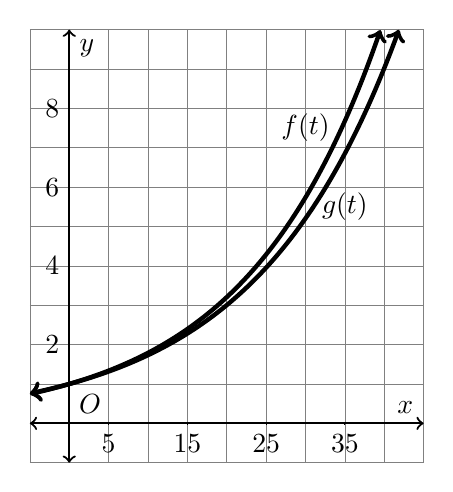
\begin{tikzpicture}[xscale=.1, yscale=.5]
		\draw[style=help lines, ystep=1, xstep=5] (-5,-1) grid (45,10);
		\draw[thick,<->] (-5,0) -- (45,0) node[anchor=south east] {$x$};
		\draw[thick,<->] (0,-1) -- (0,10) node[anchor=north west] {$y$};
		\foreach \x in {5, 15, 25, 35}
		    \draw (\x cm,1pt) -- (\x cm,-1pt) node[anchor=north] {$\x$};
		\foreach \y in {2, 4, 6, 8}
		    \draw (1pt,\y cm) -- (-1pt,\y cm) node[anchor=east] {$\y$};
		\node[anchor=south west] at (0,0) {$O$};
		\draw[<->, ultra thick, domain=-5:39.517,smooth,samples=200] plot (\x, {1.06^\x}) node at (30,7.5) {$f(t)$};
		\draw[<->, ultra thick, domain=-5:41.865,smooth,samples=200] plot (\x, {e^(0.055*\x)}) node at (35,5.5) {$g(t)$};
	\end{tikzpicture}\\
%%%%%%%%%%%%%%%%%%%%%%%%%%%%%%%%%%%%
\begin{verbatim}
%%%%%%%%%scales example%%%%%%%%%%%%%%%%%
	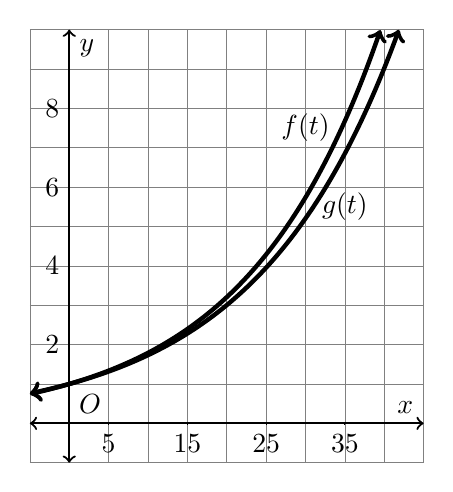
\begin{tikzpicture}[xscale=.1, yscale=.5]
		\draw[style=help lines, ystep=1, xstep=5] (-5,-1) grid (45,10);
		\draw[thick,<->] (-5,0) -- (45,0) node[anchor=south east] {$x$};
		\draw[thick,<->] (0,-1) -- (0,10) node[anchor=north west] {$y$};
		\foreach \x in {5, 15, 25, 35}
		    \draw (\x cm,1pt) -- (\x cm,-1pt) node[anchor=north] {$\x$};
		\foreach \y in {2, 4, 6, 8}
		    \draw (1pt,\y cm) -- (-1pt,\y cm) node[anchor=east] {$\y$};
		\node[anchor=south west] at (0,0) {$O$};
		\draw[<->, ultra thick, domain=-5:39.517,smooth,samples=200] plot (\x, {1.06^\x}) node at (30,7.5) {$f(t)$};
		\draw[<->, ultra thick, domain=-5:41.865,smooth,samples=200] plot (\x, {e^(0.055*\x)}) node at (35,5.5) {$g(t)$};
	\end{tikzpicture}\\
%%%%%%%%%%%%%%%%%%%%%%%%%%%%%%%%%%%%
\end{verbatim}�
\hrule

\newpage
Lorem ipsum dolor sit amet, consectetur adipisicing elit, sed do eiusmod tempor incididunt ut labore et dolore magna aliqua. Ut enim ad minim veniam, quis nostrud exercitation ullamco laboris nisi ut aliquip ex ea commodo consequat. Duis aute irure dolor in reprehenderit in voluptate velit esse cillum dolore eu fugiat nulla pariatur. Excepteur sint occaecat cupidatat non proident, sunt in culpa qui officia deserunt mollit anim id est laborum.\newpage
\bibliographystyle{te}
\end{document}